
\section{Anti-Coincidence Counter}

% General description of ACC
The ACC in the AMS-02 experiment surrounds the inner tracker inside the magnet bore \cite{ACCPaper1, ACCPaper2} (figure \ref{ACCPicture}). Their purpose is to reject unwanted events with particles entering or leaving the inner tracker from the side. Moreover the ACC is used to reduce the trigger rate when the ISS is going through an area that is overwhelmingly dominant by low energy particle flux like the South Atlantic Anomaly (SAA) \cite{ACCAsTrigger}.  \par 

% Structure
The ACC has a cylinder shape of 1.1 m in diameter and 0.83 m in height. It is composed of 16 curved scintillator (Bicron BC-414) panels with 8 mm thickness, as shown in figure \ref{ACCScintillator}. When a particle traverses the ACC panels, it emits photons by ionization energy loss in the scintillators. Then the light is absorbed by the wavelength shifting fibres (WLS, Kuraray Y-11(200)M) that are embedded into the panels, and is transported to the PMTs (Hamamatsu R5946) placed on both ends of the ACC structure.  \par

\begin{figure}[h] 
\centering   
\subfigure[] { 
\label{ACCPicture}    
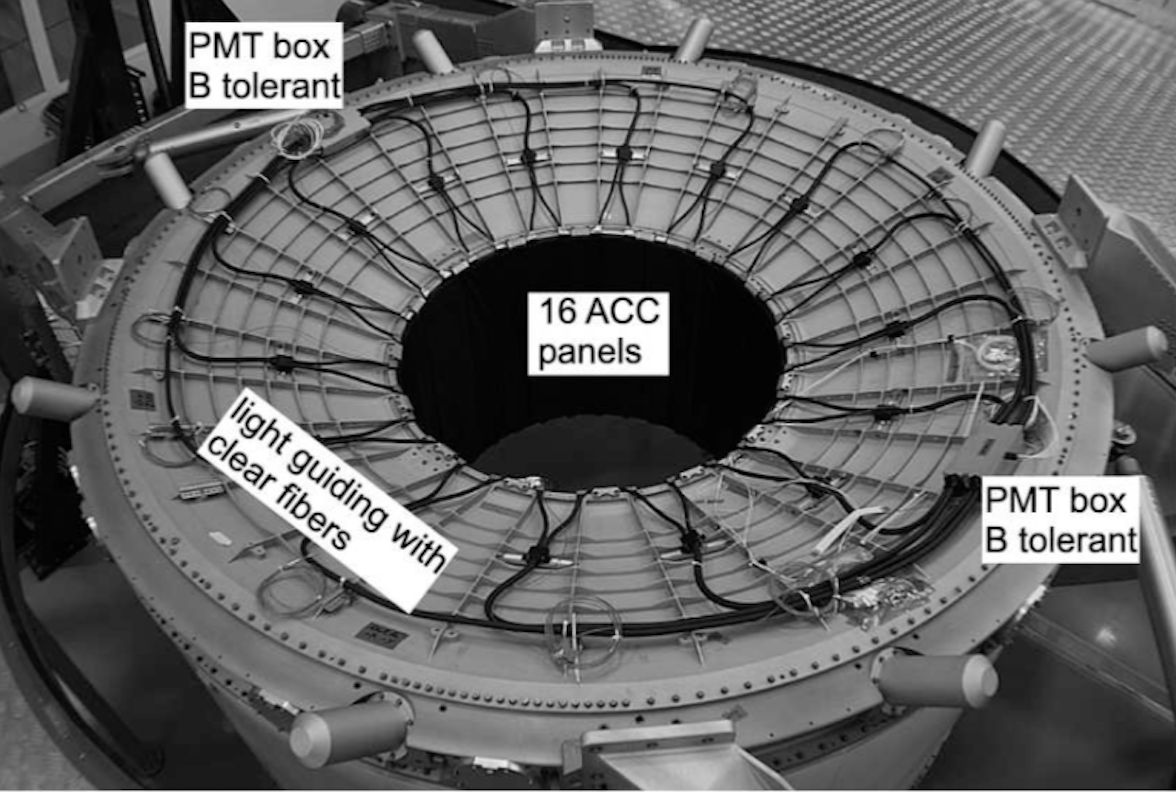
\includegraphics[width=0.52\columnwidth, height=0.29\textheight]{Figures/chapter3/ACC/UpperLeft.png} 
}    
\subfigure[] { 
\label{ACCScintillator}    
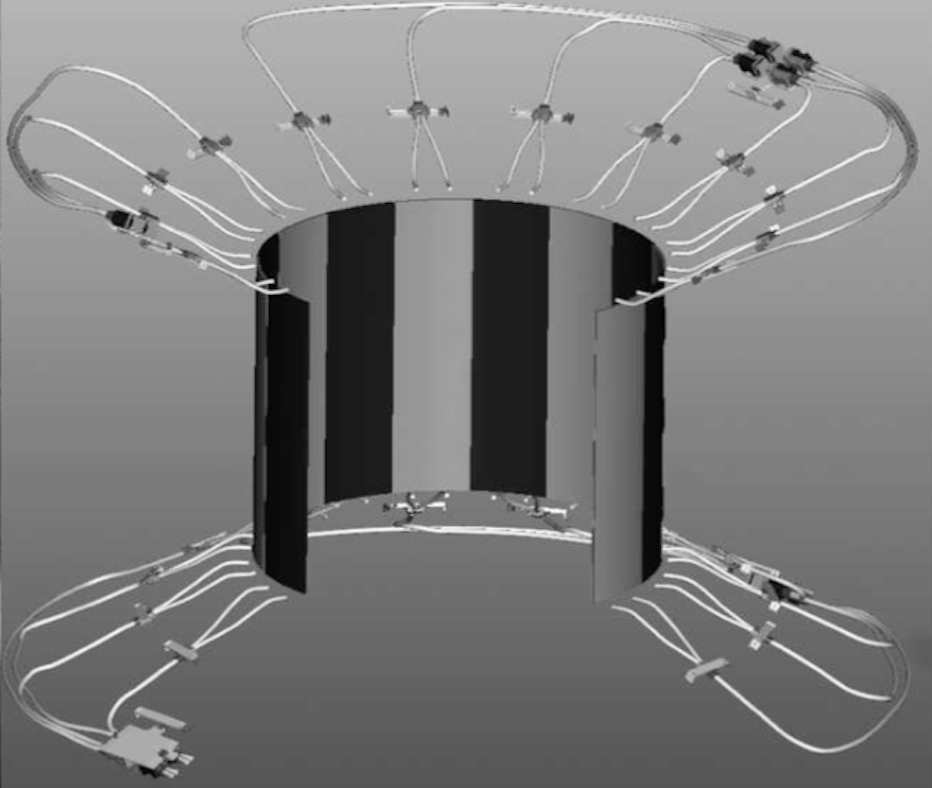
\includegraphics[width=0.40\columnwidth, height=0.29\textheight]{Figures/chapter3/ACC/UpperRight.png}    
\label{}
}    
\subfigure[] { 
\label{ACCFibers}    
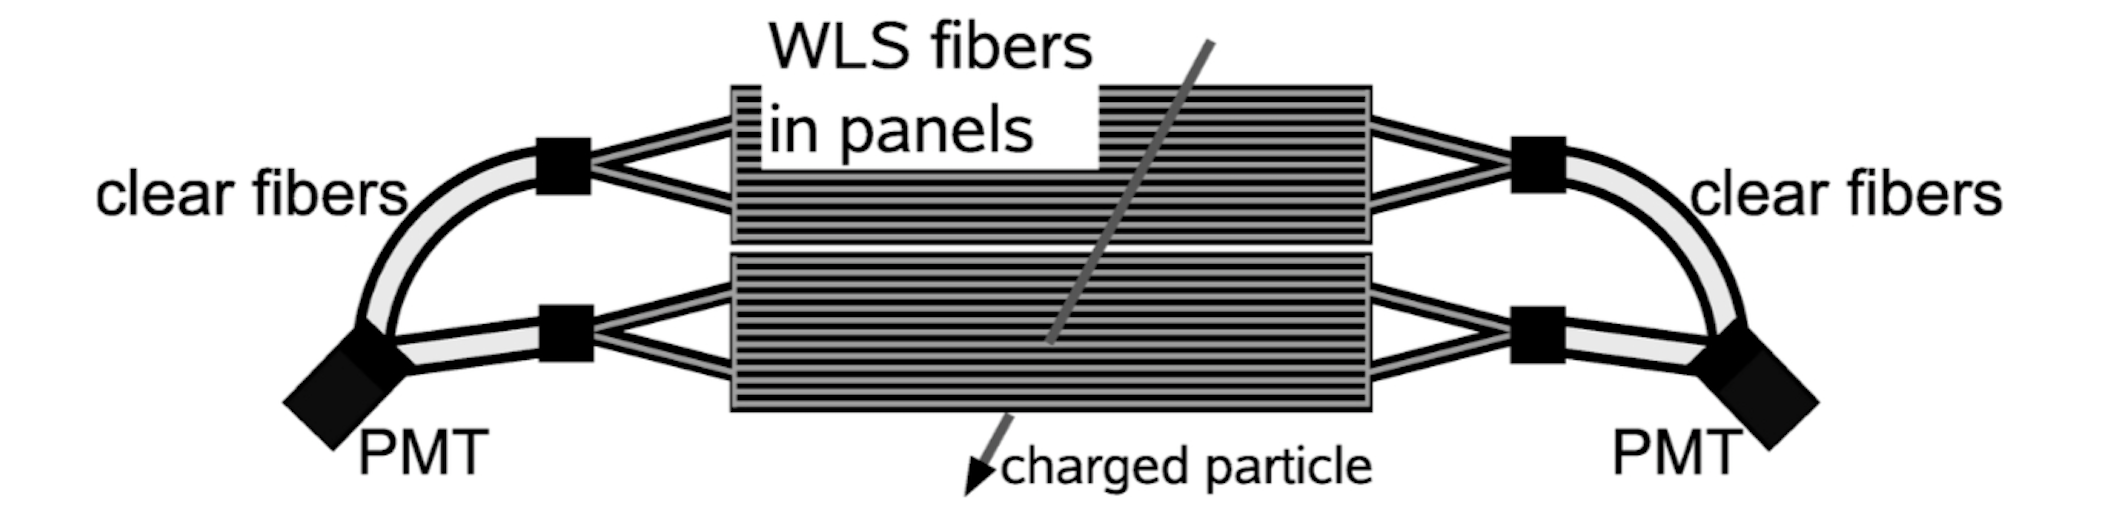
\includegraphics[width=1.0\columnwidth]{Figures/chapter3/ACC/Lower.png}    
\label{}
}    
\caption[The ACC scintillator panels pair and PMTs.]{a) The ACC system. b) The arrangement of the ACC scintillator panels. c) A panel pair and its connections to the PMTs \cite{ACCDetector}.}
\end{figure}

A pair of panels is connected to two same PMTs through clear fibers, as shown in figure \ref{ACCFibers}. This design provides redundancy capabilities and saves weight. The slot between these two panels has a tongue and a groove structure to minimize the detection inefficiency. The ACC panels efficiency has been measured at a muon test beam at CERN and found to be equal to 99.99\% \cite{AMSWebside}. \par

% Trigger
The ACC signals are used in the trigger logic to veto events with particles crossing from the side of the detector. Combined with the information from the TOF, the trigger is generated \cite{ACCAsTrigger}. 
%More details about the ACC's role in the trigger system will be given in Section \ref{TriggerEfficiencySection}.  


